\documentclass{beamer}

\usepackage[utf8]{inputenc}
\usepackage[T1]{fontenc}
\usepackage{pmboxdraw}
\usepackage{xspace}

\definecolor{darkbg}{HTML}{191959}
\definecolor{medbg}{HTML}{262686}
\definecolor{lightbg}{HTML}{3333b3}

\definecolor{tbtxl}{RGB}{0,255,0}
\definecolor{tbtxlwrap}{RGB}{0,128,0}
\definecolor{tbcomp}{RGB}{255,0,255}
\definecolor{tbklee}{RGB}{128,0,128}

\definecolor{mygreen}{rgb}{0,0.6,0}
\definecolor{mygray}{rgb}{0.5,0.5,0.5}
\definecolor{mymauve}{rgb}{0.58,0,0.82}

\definecolor{darkblue}{rgb}{0,0,.75}

\mode<presentation>
{
	\usetheme{CambridgeUS}
	
	\setbeamertemplate{navigation symbols}{}
	%\setbeamertemplate{headline}{}
	
	\usecolortheme{whale}
	\usecolortheme{orchid}
	
	%\setbeamerfont{author}{size=\scriptsize,parent=structure}
	%\setbeamerfont{institute}{size=\scriptsize,parent=structure}
	%\setbeamerfont{date}{size=\scriptsize,parent=structure}
	\setbeamerfont{title}{size={\fontsize{14}{22}},series=\bf,parent=structure}
	\setbeamerfont{footline}{size={\fontsize{6}{7}},parent=structure}
	\setbeamerfont{headline}{size={\fontsize{6}{7}},parent=structure}
	\setbeamerfont{frametitle}{size={\fontsize{14}{16}},series=\bf,parent=structure}
	\setbeamercolor{title}{bg=medbg}
	\setbeamercolor{frametitle}{fg=white,bg=medbg}
	
	%\setbeamerfont{itemize/enumerate body}{size=\scriptsize}
	%\setbeamerfont{itemize/enumerate body}{}
	%\setbeamerfont{itemize/enumerate subbody}{size=\small}
	%\setbeamerfont{itemize/enumerate subsubbody}{size=\footnotesize}
}


\usepackage{listings}
\lstset{ %
	backgroundcolor=\color{white},   % choose the background color
	basicstyle=\tiny,                % size of fonts used for the code
	breaklines=true,                 % automatic line breaking only at whitespace
	captionpos=b,                    % sets the caption-position to bottom
	commentstyle=\color{mygreen},    % comment style
	escapeinside={\%*}{*)},          % if you want to add LaTeX within your code
	keywordstyle=\color{blue},       % keyword style
	stringstyle=\color{mymauve},     % string literal style
}

\lstnewenvironment{vastcode}
{\lstset{
		basicstyle=\fontsize{6}{10}\sffamily,
		escapechar=@,
		% http://tug.ctan.org/info/symbols/comprehensive/symbols-a4.pdf
		literate =
		{/}{{$\textSFi$}}1
		{-}{{$\textSFviii$}}1
		{=}{{$\textSFii$}}1
		{|}{{$\textSFxi$}}1
	}
}
{}

\lstloadlanguages{Matlab} %use listings with Matlab for Pseudocode
\lstnewenvironment{PseudoCode}
{\lstset{
		language=Matlab,
		basicstyle=\tiny,
		keywordstyle=\color{darkblue},
		morekeywords={do,is,forall,foreach,it,map},
		escapechar=@
	}
}
{}


\newcommand{\CReconfig}{\textsc{C Reconfigurator}\xspace}

\newcommand{\id}[1]{\ensuremath{#1}}

\newcommand{\type}[1]{\id{#1}}

\newcommand{\func}[1]{\textsf{#1}}


\newcommand{\obj} [1]{\ensuremath{{\id{#1}}_?}}
\newcommand{\pc}  [1]{\ensuremath{{\id{#1}}_\phi}}
\newcommand{\lang}[1]{\ensuremath{{\id{#1}}_@}}
\newcommand{\node}[1]{\ensuremath{{\id{#1}}_\circ}}
\newcommand{\name}[1]{\textsf{#1}}
\newcommand{\lst} [1]{\ensuremath{{\id{#1}}_{::}}}

%Information to be included in the title page:
\title{\CReconfig}
\author{Alexandru F. Iosif-Lazăr}
\institute{ITU Copenhagen}
\date{26-04-2017}



\begin{document}
	
%----------------------------------------------------------------------------------------------------------------------%
%----------------------------------------------------------------------------------------------------------------------%
	\frame{\titlepage}
	
%----------------------------------------------------------------------------------------------------------------------%
%----------------------------------------------------------------------------------------------------------------------%
	\begin{frame}
		\frametitle{\CReconfig Overview}
		
		\centering
		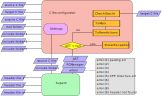
\includegraphics[height=7cm]{img/Fig1.pdf}
		
	\end{frame}

%----------------------------------------------------------------------------------------------------------------------%
%----------------------------------------------------------------------------------------------------------------------%
	\begin{frame}
	\frametitle{V-AST Syntax}
	
	\begin{columns}
		
		\column{0.5\textwidth}
		\begin{equation*}
		\label{eq:vastsyntax}
		\begin{array}{rcl}
		node & ::= & (name,list)
		\\[0.5mm]
		list & ::= & \epsilon ~\mid~ obj::list
		\\[0.5mm]
		obj & ::= & pc ~\mid~ lang ~\mid~ node
		\end{array}
		\end{equation*}
		
		\column{0.5\textwidth}
		\begin{itemize}
			\item A \type{node} is a tuple of two elements: a string \type{name} and a \type{pair} which contains the children.
			\vspace*{.5cm}
			
			\item A \type{list} can either be empty ($\epsilon$) or it can be formed of a head of type \type{obj} and a tail of type \type{list}.
			\vspace*{.5cm}
			
			\item An \type{obj} can be a presence condition \type{pc}, a language element \type{lang} or a \type{node}.
		\end{itemize}
	\end{columns}
\end{frame}


%----------------------------------------------------------------------------------------------------------------------%
%----------------------------------------------------------------------------------------------------------------------%
\begin{frame}
\frametitle{V-AST vs. Java/Xtend}

\begin{table}
\centering
\begin{tabular}{| r | l |}
	\hline
	\textbf{V-AST} & \textbf{Java/Xtend} \\\hline
	\type{obj}  & Object \\\hline
	\type{pc}   & PresenceCondition \\\hline
	\type{lang} & Language<CTag> \\\hline
	\type{node} & GNode \\\hline
	\type{list} & Pair<Object> \\\hline
\end{tabular}
\caption{Mapping from V-AST vertices to Java classes.}
\end{table}

\end{frame}


%----------------------------------------------------------------------------------------------------------------------%
%----------------------------------------------------------------------------------------------------------------------%
\begin{frame}[fragile]
\frametitle{Rule structure}

\begin{lstlisting}[language=java]
abstract class Rule {

  def init() {
    this
  }

  def dispatch PresenceCondition transform(PresenceCondition cond) {
    throw new UnsupportedOperationException("TODO: auto-generated method stub")
  }

  def dispatch Language<CTag> transform(Language<CTag> lang) {
    throw new UnsupportedOperationException("TODO: auto-generated method stub")
  }

  def dispatch Pair<Object> transform(Pair<Object> pair) {
    throw new UnsupportedOperationException("TODO: auto-generated method stub")
  }

  def dispatch Object transform(GNode node) {
    throw new UnsupportedOperationException("TODO: auto-generated method stub")
  }	
}
\end{lstlisting}

\end{frame}


%----------------------------------------------------------------------------------------------------------------------%
%----------------------------------------------------------------------------------------------------------------------%
\begin{frame}[fragile]
\frametitle{Other rule types}

\begin{lstlisting}[language=java]
abstract class Rule {

}

//--------------------------------------------------------

abstract class AncestorGuaranteedRule extends Rule {

  protected var ArrayList<GNode> ancestors
  
  // Returns the presence condition guarding the node from the bottom-most Conditional ancestor.
  def protected PresenceCondition guard(Node node) { ... }
  
  // Computes the conjunction of all ancestor PresenceConditions of a Node.
  def protected PresenceCondition presenceCondition(Node node) { .. }

}

//--------------------------------------------------------

abstract class ScopingRule extends AncestorGuaranteedRule {

  // Collects declarations as it traverses the AST top-bottom until the place where it can be applied.
  protected val DeclarationScopeStack variableDeclarations
  protected val DeclarationPCMap typeDeclarations
  protected val DeclarationPCMap functionDeclarations

}
\end{lstlisting}

\end{frame}


%----------------------------------------------------------------------------------------------------------------------%
%----------------------------------------------------------------------------------------------------------------------%
\begin{frame}[fragile]
\frametitle{Strategy}
\begin{lstlisting}[language=java]
abstract class Strategy {

  protected val ArrayList<Rule> rules

  new() {
    this.rules = new ArrayList<Rule>
  }

  def register(Rule rule) {
    rules.add(rule.init())
  }

  def dispatch PresenceCondition transform(PresenceCondition cond) {
    throw new UnsupportedOperationException("TODO: auto-generated method stub")
  }

  def dispatch Language<CTag> transform(Language<CTag> lang) {
    throw new UnsupportedOperationException("TODO: auto-generated method stub")
  }

  def dispatch Pair<Object> transform(Pair<Object> pair) {
    throw new UnsupportedOperationException("TODO: auto-generated method stub")
  }

  def dispatch Object transform(GNode node) {
    throw new UnsupportedOperationException("TODO: auto-generated method stub")
  }

}
\end{lstlisting}
\end{frame}


%----------------------------------------------------------------------------------------------------------------------%
%----------------------------------------------------------------------------------------------------------------------%
\begin{frame}[fragile]
\frametitle{Other Strategy types}
\begin{lstlisting}[language=java]
abstract class Strategy {

  protected val ArrayList<Rule> rules

  new() { this.rules = new ArrayList<Rule> }

  def register(Rule rule) {
    rules.add(rule.init())
  }
}

//--------------------------------------------------------

abstract class AncestorGuaranteedStrategy extends Strategy {

  protected val ArrayList<GNode> ancestors

  new() {
    super()
    this.ancestors = new ArrayList<GNode> }

  public def register(AncestorGuaranteedRule rule) {
    rules.add(rule.init(ancestors))
  }
}

//--------------------------------------------------------

class TopDownStrategy extends AncestorGuaranteedStrategy {

}
\end{lstlisting}
\end{frame}


%----------------------------------------------------------------------------------------------------------------------%
%----------------------------------------------------------------------------------------------------------------------%
\begin{frame}[fragile]
\frametitle{Immutable AST}

	\begin{columns}
	
	\column{0.33\textwidth}
	\begin{vastcode}
@\node{\name{DeclarationOrStatementList}}@
/ @\node{\name{Conditional}}@
| - @\id{\psi}@
| - @\node{\name{Conditional}}@
| | - @\id{\phi_1}@
| | = @\lst{\id{children_1}}@
| = @\node{\name{Conditional}}@
|   - @\id{\phi_2}@
|   = @\lst{\id{children_2}}@
= @\lst{\id{tail}}@
	\end{vastcode}
	
	\column{0.33\textwidth}
	\begin{vastcode}
@\color{blue}\node{\name{DeclarationOrStatementList}}@
/ @\color{blue}\node{\name{Conditional}}@
| - @\color{blue}\id{\phi_1} $\land$ \id{\psi}@
| = @\lst{\id{children_1}}@
- @\color{blue}\node{\name{Conditional}}@
| - @\color{blue}\id{\phi_2} $\land$ \id{\psi}@
| = @\lst{\id{children_2}}@
= @\lst{\id{tail}}@
	\end{vastcode}
	
	\column{0.33\textwidth}
	assuming \\
	\id{\phi_2} $\land$ \id{\psi} = \pc{true}
	\begin{vastcode}
@\color{red}\node{\name{DeclarationOrStatementList}}@
/ @\color{blue}\node{\name{Conditional}}@
| - @\color{blue}\id{\phi_1} $\land$ \id{\psi}@
| = @\lst{\id{children_1}}@
- @\lst{\id{children_2}}@
= @\lst{\id{tail}}@
	\end{vastcode}
	
	\end{columns}
\end{frame}


%----------------------------------------------------------------------------------------------------------------------%
%----------------------------------------------------------------------------------------------------------------------%
\begin{frame}[fragile]
\frametitle{Top-Down Strategy I}
	
	\begin{columns}
	
	\column{0.5\textwidth}
	
	\begin{PseudoCode}
@\type{pc}@ transform (@\type{pc} \pc{cond}@)
  @\pc{newCond} = \pc{cond}@
  rules.foreach[rule |
    @\pc{newCond} = rule.transform(\pc{newCond})@
  ]
  return @\pc{newCond}@
	\end{PseudoCode}

	\column{0.5\textwidth}

	\begin{PseudoCode}
@\type{lang}@ transform (@\type{lang} \lang{lang}@)
  @\lang{newLang} = \lang{lang}@
  rules.foreach[rule |
    @\lang{newLang} = rule.transform(\lang{newLang})@
  ]
  return @\pc{newLang}@
	\end{PseudoCode}
	
	\end{columns}
	
\end{frame}


%----------------------------------------------------------------------------------------------------------------------%
%----------------------------------------------------------------------------------------------------------------------%
\begin{frame}[fragile]
\frametitle{Top-Down Strategy II}

\begin{columns}
	
	\column{0.5\textwidth}
	
	\begin{PseudoCode}
@\type{obj}@ transform (@\type{node} \node{node}@)
  @\node{newNode} = \node{node}@
  do @\node{prev} = \node{newNode}@
    rules.foreach[rule |
      @\node{newNode}@ = rule.transform(@\node{newNode}@)
    ]
    
    if (@\node{newNode} : (\name{NodeName},\lst{children})@)
      @\node{ancestor} = \node{newNode}@
      ancestors.add(@\node{ancestor}@)
      @\node{newNode}@ = (@\name{NodeName}@,transform(@\lst{children}@))
      ancestors.remove(@\node{ancestor}@)
      if (@\node{ancestor} != \node{newNode}@)
        return @\node{newNode}@
  while (@\node{newNode} != \node{prev}@)
  return @\node{newNode}@
	\end{PseudoCode}
	
	\column{0.5\textwidth}
	
	\begin{PseudoCode}
@\type{list}@ transform (@\type{list} \lst{list}@)
  if (@\lst{list}@ != @$\epsilon$@)
    @\lst{newList} = \lst{list}@
    do @\lst{prev} = \lst{newList}@
      rules.foreach[rule |
        @\lst{newList}@ = rule.transform(@\lst{newList}@)
      ]

    if (@\lst{newList} != \lst{prev}@)
      return @\lst{newList}@
      
    if (@\lst{newList} : \obj{head}::\lst{tail}@)
      @\obj{newHead}@ = transform(@\obj{head}@)
      @\lst{newList}@ = transform(@\lst{tail}@)
      
      if (@\obj{newHead}@ != @\obj{head}@ || @\lst{newList}@ != @\lst{tail}@)
        return @\obj{newHead}@::@\lst{newList}@
      else
        return @\lst{newList}@
\end{PseudoCode}
	
\end{columns}

\end{frame}


%----------------------------------------------------------------------------------------------------------------------%
%----------------------------------------------------------------------------------------------------------------------%
\begin{frame}[fragile]
\frametitle{RemOneRule}

\noindent
\begin{tabular}{| p{.2\textwidth} | p{.2\textwidth} | p{.6\textwidth} |}
	\hline
	Input \lst{\id{list}} & Output \lst{\_} & Algorithm \\\hline

\begin{vastcode}
/ @\node{\name{Conditional}}@
| - @\pc{\name{true}}@
| = @\lst{\id{children}}@
= @\lst{\id{tail}}@
\end{vastcode} &

\begin{vastcode}
/ @\lst{\id{children}}@
= @\lst{\id{tail}}@
\end{vastcode} &

\begin{PseudoCode}
preconditions:
  @\lst{\id{list}} != $\epsilon$@
  @\lst{\id{list}}.\func{head}@ : (@\name{Conditional}@,@\_@)
  @\lst{\id{list}}.\func{head}@.filter(@\type{pc}@).size = 1
  @\lst{\id{list}}.\func{head}@[0] = @\pc{\name{true}}@

do:
  return @\lst{\id{list}}.\func{head}@
    @.\func{getChildrenGuardedBy}(\pc{\name{true}})@
    @.\func{append}(\lst{\id{list}}.\func{tail})@
\end{PseudoCode} \\\hline
\end{tabular}
\end{frame}


%----------------------------------------------------------------------------------------------------------------------%
%----------------------------------------------------------------------------------------------------------------------%
\begin{frame}[fragile]
\frametitle{RemZeroRule}

\noindent
\begin{tabular}{| p{.2\textwidth} | p{.2\textwidth} | p{.6\textwidth} |}
	\hline
	Input \lst{\id{list}} & Output \lst{\_} & Algorithm \\\hline
	
\begin{vastcode}
/ @\node{\name{Conditional}}@
| - @\pc{\name{false}}@
| = @\lst{\id{children}}@
= @\lst{\id{tail}}@
\end{vastcode} &

\begin{vastcode}
@\lst{\id{tail}}@
\end{vastcode} &
	
\begin{PseudoCode}
preconditions:
  @\lst{\id{list}} != $\epsilon$@
  @\lst{\id{list}}.\func{head}@ : (@\name{Conditional}@,@\_@)
  @\lst{\id{list}}.\func{head}@.filter(@\type{pc}@).size = 1
  @\lst{\id{list}}.\func{head}@[0] = @\pc{\name{false}}@
	
do:
  return @\lst{\id{list}}.\func{tail}@
\end{PseudoCode} \\\hline
\end{tabular}
\end{frame}


%----------------------------------------------------------------------------------------------------------------------%
%----------------------------------------------------------------------------------------------------------------------%
\begin{frame}[fragile]
\frametitle{SplitConditionalRule}

\noindent
\begin{tabular}{| p{.2\textwidth} | p{.2\textwidth} | p{.6\textwidth} |}
\hline
Input \lst{\id{list}} & Output \lst{\_} & Algorithm \\\hline

\begin{vastcode}
/ @\node{\name{Conditional}}@
| - @\id{\phi_1}@
| - @\lst{\id{children_1}}@
| - @\id{\phi_2}@
| - @\lst{\id{children_2}}@
| - @\id{\phi_n}@
| = @\lst{\id{children_n}}@
= @\lst{\id{tail}}@
\end{vastcode} &

\begin{vastcode}
/ @\node{\name{Conditional}}@
| - @\id{\phi_1}@
| = @\lst{\id{children_1}}@
- @\node{\name{Conditional}}@
| - @\id{\phi_2}@
| = @\lst{\id{children_2}}@
- @\node{\name{Conditional}}@
| - @\id{\phi_n}@
| = @\lst{\id{children_n}}@
= @\lst{\id{tail}}@
\end{vastcode} &

\begin{PseudoCode}
preconditions:
  @\lst{\id{list}} != $\epsilon$@
  @\lst{\id{list}}.\func{head}@ : (@\name{Conditional}@,@\_@)
  @\lst{\id{list}}.\func{head}@.filter(@\type{pc}@).size >= 2

do:
  @\lst{\id{newList}} = $\epsilon$@

  for @(\id{\phi_i} in [\id{\phi_1}..\id{\phi_n}])@
    @\lst{\id{newList}} = \lst{\id{newList}}.\func{append}(@
      @(\name{Conditional},@
      @\id{\phi_i}::\lst{\id{list}}.\func{head}.\func{getChildrenGuardedBy}(\id{\phi_i})))@

  return @\lst{\id{list}}.\func{tail}@
\end{PseudoCode} \\\hline
\end{tabular}
\end{frame}


%----------------------------------------------------------------------------------------------------------------------%
%----------------------------------------------------------------------------------------------------------------------%
\begin{frame}[fragile]
\frametitle{ConstrainNestedConditionalsRule}

\noindent
\begin{tabular}{| p{.2\textwidth} | p{.3\textwidth} | p{.5\textwidth} |}
\hline
Input \node{\id{node}} & Output \node{\_} & Algorithm \\\hline

\begin{vastcode}
ancestors:
@(\name{Conditional},\id{\psi_1}::\lst{\_})@
@(\name{Conditional},\id{\psi_2}::\lst{\_})@
@(\name{Conditional},\id{\psi_n}::\lst{\_})@

@\node{\name{Conditional}}@
- @\id{\phi_1}@
= @\lst{\id{children}}@
\end{vastcode} &

\begin{vastcode}
@\node{\name{Conditional}}@
- @\func{constrain}(\id{\phi_1}, $\id{\psi_1} \land \id{\psi_2} \land \id{\psi_n}$)@
= @\lst{\id{children}}@
\end{vastcode} &

\begin{PseudoCode}
preconditions:
@\node{\id{node}}.\func{name} = \name{Conditional}@
@\node{\id{node}}@.filter(@\type{pc}@).size = 1
	
do:
@\pc{\id{simpl}} = \func{constrain}(\id{\phi}, \node{\id{node}}.\func{presenceCondition})@

if @(\pc{\id{simpl}} != \id{\phi})@
  return @(\name{Conditional},\pc{\id{simpl}}::\node{\id{node}}.\func{toList}.\func{tail})@
else
  return @\node{\id{node}}@
\end{PseudoCode} \\\hline
\end{tabular}
\end{frame}


%----------------------------------------------------------------------------------------------------------------------%
%----------------------------------------------------------------------------------------------------------------------%
\begin{frame}[fragile]
\frametitle{ConditionPushDownRule}

\noindent
\begin{tabular}{| p{.25\textwidth} | p{.2\textwidth} | p{.55\textwidth} |}
\hline
Input \lst{\id{list}} & Output \lst{\_} & Algorithm \\\hline

\begin{vastcode}
/ @\node{\name{Conditional}}@
| - @\id{\psi_1}@
| - @\node{\name{Conditional}}@
| | - @\id{\phi_{11}}@
| | = @\lst{\id{children_{11}}}@
| - @\id{\psi_2}@
| - @\node{\name{Conditional}}@
| | - @\id{\phi_{21}}@
| | - @\lst{\id{children_{21}}}@
| | - @\id{\phi_{22}}@
| | = @\lst{\id{children_{22}}}@
| - @\node{\name{Conditional}}@
| | - @\id{\phi_{31}}@
| | = @\lst{\id{children_{31}}}@
| - @\id{\psi_n}@
| = @\node{\name{Conditional}}@
|   - @\id{\phi_{n1}}@
|   = @\lst{\id{children_{n1}}}@
= @\lst{\id{tail}}@
\end{vastcode} &

\begin{vastcode}
/ @\node{\name{Conditional}}@
| - @$\id{\phi_{11}} \land \id{\psi_1}$@
| = @\lst{\id{children_{11}}}@
- @\node{\name{Conditional}}@
| - @$\id{\phi_{21}} \land \id{\psi_2}$@
| - @\lst{\id{children_{21}}}@
| - @$\id{\phi_{22}} \land \id{\psi_2}$@
| = @\lst{\id{children_{22}}}@
- @\node{\name{Conditional}}@
| - @$\id{\phi_{31}} \land \id{\psi_2}$@
| = @\lst{\id{children_{31}}}@
- @\node{\name{Conditional}}@
| - @$\id{\phi_{n1}} \land \id{\psi_n}$@
| = @\lst{\id{children_{n1}}}@
= @\lst{\id{tail}}@
\end{vastcode} &

\begin{PseudoCode}
preconditions:
@\lst{\id{list}} != $\epsilon$@
@\lst{\id{list}}.\func{head}@ : @(\name{Conditional},\_)@
@\lst{\id{list}}.\func{head}@.forall[it:@\pc{\_} $\lor$ @it:@(\name{Conditional},\_)@]

do:
@\lst{\id{list}}.\func{head}@.filter(@\type{cond}@).map[@\node{node}@ | 
  (@\name{Conditional},\node{node}@.map[@\obj{child}@ |
    if (@\obj{child}@ : @\pc{\_}@) @\pc{child} $\land$ \func{pcOf}(\node{node})@
    else @\obj{child}@
  ])
].@\func{append}(\lst{\id{tail}})@
\end{PseudoCode} \\\hline
\end{tabular}
\end{frame}


%----------------------------------------------------------------------------------------------------------------------%
%----------------------------------------------------------------------------------------------------------------------%
\begin{frame}[fragile]
\frametitle{MergeSequentialMutexConditionalRule}

\noindent
\begin{tabular}{| p{.2\textwidth} | p{.2\textwidth} | p{.6\textwidth} |}
\hline
Input \lst{\id{list}} & Output \lst{\_} & Algorithm \\\hline

\begin{vastcode}
/ @\node{\name{Conditional}}@
| - @\id{\phi_1}@
| = @\lst{\id{children_1}}@
- @\node{\name{Conditional}}@
| - @\id{\phi_2}@
| = @\lst{\id{children_2}}@
= @\lst{\id{tail}}@
\end{vastcode} &

\begin{vastcode}
/ @\node{\name{Conditional}}@
| - @\id{\phi_1} $\lor$ \id{\phi_2}@
| = @\lst{\id{children_1}}@
= @\lst{\id{tail}}@
\end{vastcode} &

\begin{PseudoCode}
preconditions:
  @\lst{\id{list}} != $\epsilon$@
  @\lst{\id{list}}.\func{size} >= 2@
  @\lst{\id{list}}.\func{head}@ : @(\name{Conditional},\_)@
  @\lst{\id{list}}.\func{head}@.filter(@\type{cond}@).@\func{size}@ == 1
  @\lst{\id{list}}.\func{tail}.\func{head}@ : @(\name{Conditional},\_)@
  @\lst{\id{list}}.\func{tail}.\func{head}@.filter(@\type{cond}@).@\func{size}@ == 1
  @\func{areMutex}(\id{\phi_1},\id{\phi_2})@
  @\func{structurallyEquals}(\lst{\id{children_1}},\lst{\id{children_2}})@

do:
  @(\name{Conditional}, \id{\phi_1} $\lor$ \id{\phi_2} :: \lst{\id{children_1}}) :: \lst{\id{tail}}@
\end{PseudoCode} \\\hline
\end{tabular}
\end{frame}
	
\end{document}